\documentclass{article} % For LaTeX2e
\usepackage{nips12submit_e,times}
\usepackage{amsmath}
\usepackage{graphicx}
\usepackage{caption}
\usepackage{subcaption}
\usepackage{comment}
\usepackage{hyperref}
\usepackage{url}
\usepackage[top=1.0in, bottom=1.0in, left=1.0in, right=1.0in]{geometry}

%\renewcommand\refname{Papers To Read}
\title{Semantic Segmentation Using Label Propagation}

\author{
Aravindh Mahendran \\
\texttt{amahend1@andrew.cmu.edu} \\ 
\And
Nitish Thatte \\
\texttt{nitisht@andrew.cmu.edu} \\
\AND
Adwait Gandhe \\
\texttt{agandhe@andrew.cmu.edu} \\
}

\newcommand{\fix}{\marginpar{FIX}}
\newcommand{\new}{\marginpar{NEW}}

\nipsfinalcopy

\begin{document}
\maketitle

\begin{abstract}
Semantic image segmentation is the process of assigning human relevant labels to pixels in an image and is a high level vision problem. In this work we attempt a supervised learning approach to solve this problem by training a classifier that helps propagate labels to improve upon a prior distribution over semantic labels. We present our results on the 13 class MSRC V1 Dataset. We achieved an accuracy of $56.88\%$ across all test images and an improvement in accuracy of $0.17\%$ over our prior segmentations.
\end{abstract}

\section{Introduction}
Semantic segmentation is the process of assigning a class label to each pixel of the image. This is an important problem in computer vision for understanding the underlying information in an image. While classical segmentation techniques group together the pixels based on low level features, semantic segmentation adopts a supervised learning approach. There are two common methods for semantic segmentation. The first makes use of low level features and combines them with a learning framework to obtain higher level labels. The second approach is to use low level cues, rather than features, with random fields and learn a unified framework using low level segmentation. In this paper, present a novel approach that improves upon a prior distribution obtained using a bag of visual words over mean-shift segments by propagating labels at the discretion of a trained Random Forest \cite{Statistics01randomforests}.

This paper is structured as follows: Section \ref{sec:Related} talks about the related work. Section \ref{sec:Problem} discusses the problem statement. Section \ref{sec:Proposed} discusses our method for semantic image segmentation. We present the experiments conducted and the results obtained in section \ref{sec:Exp}. Finally we summarize our conclusions in section \ref{sec:Conclusion}.
\label{sec:Intro}

\subsection{Related Work}
\label{sec:Related}
One of the first approaches for semantic segmentation utilized an Implicit Shape Model%TODO @Adwait
\cite{Leibe04combinedobject}. 
Another approach used a generative model based on the bag of words representation for such simultaneous recognition and segmentation \cite{cao:spatially}.  
Furthermore, a method based on some of these approaches for scoring low-level patches according to their class relevance and propagating these posterior probabilities to pixels has been developed \cite{conf/bmvc/CsurkaP08}.

Several recent approaches use random fields to incorporate local cues without implementing low level segmentation. For example, \cite{Kumar:2005:OC:1068507.1068889} proposes a Bayesian method for combining top-down and bottom-up cues. Conditional random fields have also been used for this purpose \cite{Kumar:2005:HFF:1097115.1097790} \cite{Richard04multiscaleconditional}. Finally, Textonboost \cite{Shotton06textonboost:joint} is an approach to learning a discriminative model of object classes incorporating appearance, shape and context information efficiently. We suggest \cite{SegmentRegionsParts} for a review of other semantic image segmentation approaches.

A third class of algorithms propagate labels given a prior estimate of the segmentation. One of the recent approaches, that inspired our work, used a distance metric in feature space along with %TODO @nitish

%------------------------------------------------------------------------------------------

\subsection{Problem Definition}
\label{sec:Problem}
Semantic segmentation requires assigning a label $l \in L$ to each pixel in an image, where $L$ is a set of pre decided labels. In the supervised version of this problem we are given a collection of hand labeled training images and are required to predict labels for every pixel in a new test image. 

%------------------------------------------------------------------------------------------
\section{Proposed Method}
\label{sec:Proposed}
\subsection{Intuition}
\label{sec:intuition}
To perform semantic segmentation, one normally wants to divide the image into regions based on image statistics and then categorize these regions into semantic classes. If one uses big regions, object boundaries are often missed and the segmentation output is smudged. On the other hand, if small regions are used, features within these are too noisy to perform reliable classification resulting in low accuracy. A good trade off between the two is hard to achieve. Therefore, an approach that makes uncertain decision on big patches and less complex decisions on small patches should yield good results. 

\subsection{Our Approach}
Based on the above intuition and the idea of label propagation we propose a two phase algorithm. In the first step we process big patches generated by mean-shift segmentation to obtain $P(label | feature)$. In the second step, we decide whether two small patches should have the same label or not and propagate labels based on this decision. This second step corrects for the fact that the prior acting on large patches may miss small details. Further, the second step is less prone to noise because the task of deciding whether to propagate a label reduces to binary classification instead of $|L|$ classification.
\subsubsection{Features}
\paragraph{Textons}
Textons represent texture information.
A collection of filters is used to process each pixel to obtain a per
pixel feature vector.
This is quantized to a single number by selecting a vector nearest to the
current one from a precomputed dictionary of feature cluster centers.
If each vector in this dictionary is considered to be a word, this
representation gives one word per image pixel and is called the TextonMap
or WordMap. %TODO: Insert figure
A bag of words histogram is computed for each super pixel or segment by
counting word occurrences.
Texture information is more reliable over large regions because of inseparability of data at small scales.
We used the filter bank and dictionary provided by \cite{malisiewicz-cvpr08}.

\paragraph{Color}
Color information is important for separating classes that lack texture or
have similar texture.
We use the per channel color histogram, color mean and standard deviation
from the HSV color space.
Color information is more reliable at small scales because large regions show too much intra class variability.

\subsubsection{Baseline}
\label{baseline}
Label propagation requires an initial estimate of the semantic class of each pixel. In our approach we further require an estimate of this classifications' uncertainty. This initial estimate is based on big mean-shift patches using texture information. This follows from our intuition of looking at large patches in the first phase and that textons are more reliable over large patches.
\paragraph{Training} Each training image is divided into segments using
Mean-shift based EDISON \cite{meanshift}.
A normalized texton histogram (bag of words representation) is computed for each segment.
The ground truth label for each segment is selected by taking a majority vote over per pixel ground truth labels.

\paragraph{Testing} For each test image, mean-shift segments and normalized texton histograms of the same are computed.
A new model is trained from the k-most similar images to the test image. Similarity here is measured by euclidean distance between GIST \cite{Gist} feature representations of images. Not training on the entire training set gives a great boost to test accuracy.
The probability distribution $P(Label | feature)$ is computed by counting the occurrences of each label in the K nearest segments from the training data.
This distribution is copied to each pixel in the segment and a per pixel distribution and entropy is thus available.

\subsubsection{Label Propagation}
Label propogation will now try to improve upon the baseline (or prior), by training a random forest that predicts whether two super pixels share the same label and propagating labels whenever this prediction contradicts the baselines output.
This requires that the image be divided into small regions (super pixels) and also requires the construction of a super pixel connectivity graph, the edges of which will be queries given to the random forest.
\paragraph{Super pixels and connectivity graph}
\label{sec:labprop}
Each image is divided into super pixels at two different scales such that
the coarse super pixels align with corresponding finer ones.
This is achieved by using \cite{}.%TODO Cite the super pixel people.
A graph is constructed where each fine super pixel is connected to its
direct neighborhood and to all fine super pixels inside the same
coarse super pixel.
The later of these connections ensure that we have more long range propogation. This is important because some parts of objects are hard to classify as corresponding to that object class without having observed the other parts.

\paragraph{Training the classifier}
We train a classifier that decides whether or not two super pixels should
have the same label.
We assign a label for each super pixel by taking the majority vote over
ground truth labels of each pixel in it.
Each edge in the super pixel graph of a training image is considered a
positive sample if corresponding super pixels have the same label,
negative other wise.
This training data is collected over the k nearest neighbors to the test
image and used to train a random forest.
If done this way, we have too many positive samples and too few negatives
and discriminative learning fails to separate them.
We resample the training data to ensure a low enough ratio between these
before training our classifier.
Note that we train a new random forest for every test image.
Texton and color features are concatenated to describe each super pixel.
Further, each edge in the graph is described by the absolute difference of super pixel features.

\paragraph{Propagating Labels}
The baseline algorithm provides a probability for each pixel label pair. Averaged over all pixels within a super pixel we obtain the distribution for each super pixel.
The entropy for each super pixel can be calculated from this distribution.
The label with highest probability is treated as the label assigned to
each pixel.
A majority vote over this assignment is used to determine the label for
each super pixel.
When the baseline is inconsistent with the prediction of our random
forest, we propagate labels from the super pixel with lower entropy to
the super pixel with higher entropy.
This propagation is run from the lowest entropy super pixel to the highest
entropy super pixel propagating labels to super pixels further down in
this sorted list.

\subsection{Other Attempted Methods}
\subsubsection{HMLN}
Markov Logic Networks \cite{Domingos06unifyinglogical} \cite{Richardson06markovlogic} attach weights to first-order logic formulae and view them as templates for building Markov Networks. Hybrid Markov Logic Networks (HMLNs)\cite{wang2008hybrid} are an extension that allow for continuous properties to appear as features. Hybrid Markov Logic Networks combine logic and probabilistic inference techniques. This provides a powerful tool for solving high level problems such as semantic segmentation which involve complexity and noise. Our initial approach till the mid term report was based on an implementation of this tool called Alchemy \cite{alchemy}. This attempt, however, failed due to bugs in the implementation and memory issues causing lack of scalability to our dataset. We also attempted to use the software ProbCog \cite{progcog}, however the software did not allow continuous properties to appear as features and we had to abandon the approach. 

\subsubsection{SVM for Label Propagation}
We experimented with SVM's in place of random forests and found them to not converge when training on the entire dataset. Training on the nearest neighbors of a test image lead to convergence but the results were too bad to be used. We experimented with linear, quadratic and radial basis function kernels.

\subsubsection{Conditional Random Fields}
Conditional random fields \cite{lafferty2001conditional} are undirected graphical models that can perform inference to compute marginal distributions of label probabilities given features.
We attempted to use these for generating baseline segmentations using the Ising model with each pixel as a node.
These, however, are computationally expensive as they have loops.
We experimented with pseudo log likelihood training and loopy belief propogation using the UGM toolbox\cite{UGMSoftware}.
The maximum aposteriori estimate of label assignments to image pixels always labeled each pixel as Grass.
This was due to a very high unary potential learnt for the corresponding node. 
We did not pursue this approach due to very high computational requirements.
Furthermore, loopy belief propogation did not converge after more than 6 hours of training on a small subset of the images.

\subsection{Adaboost}
Another classifier that we tried was Adaboost \cite{Freund96experimentswith}. Adaboost is well suited for our application because, if each weak classifier deals with only a subset of the features, it will perform feature selection. The results on the classification task were, however, not significantly different from Random Forests. This may be because feature selection is also the intuition behind random forests as each tree in the forest acts on a random subset of the feature set. Furthermore, the run time for training and testing was significantly higher when using Adaboost and infeasible given the size of our dataset and computational resources.
%------------------------------------------------------------------------------------------


%------------------------------------------------------------------------------------------
\section{Experiments}
\label{sec:Exp}

We tested our algorithm on the MSRC V1 Dataset \cite{MSRC}, which we randomly split into 120 test images and 120 training images.
We tested our algorithm to quantify the improvement over the prior segmentation that the label propagation method provided. We also examined the performance gain from training both the random forest and bag of words model on the $k$-NN versus training on all the images.

\subsection{Cross Validation}
\label{sec:cross}

To optimize our algorithm we performed leave-one-out cross validation. We chose this particular style of cross-validation because our algorithm requires retraining the random forest for each test image. Thus, all forms of $k$-fold cross validation reduce to leave-one-out validation for our method.

The cross validation parameters that needed to be optimized were $k_{bag}$ for the $k$-nearest-neighbor images from which the bag of words model is computed, $k_{hist}$ for the $k$-nearest-neighbor Texton histograms from which the distribution $P(Label | feature)$ is generated, $k_{forest}$ for the $k$-nearest-neighbors used by the random forest, and a ratio parameter used to balanced the number true and false edges on the connectivity graph. 

Due to a lack of computational resources, optimizing these four parameters simultaneously proved intractable. Therefore, the we assumed that the parameters for the bag-of-words model and the random forest affect the final segmentation independently. This assumption is supported by the relative magnitudes by which the parameters affect the accuracy of the semantic segmentation

\begin{figure}[htb]
\centering
	\begin{subfigure}[t]{0.33\textwidth}
		\centering
		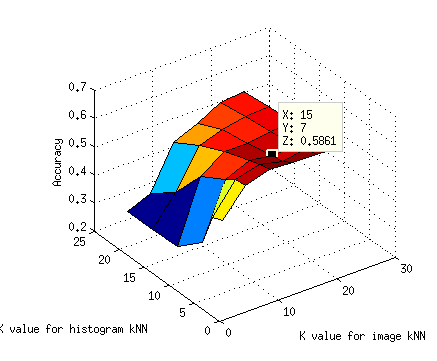
\includegraphics[width = \textwidth]{./img/pickK}
		\parbox{.95\textwidth}{\caption{Accuracy versus bag of words model parameters obtained from leave-one-out cross validation. The chosen parameters $k_{imgs} = 15$, and $k_{histo} = 7$ are highlighted. \label{fig:Kbag} }}
			\end{subfigure}
	\begin{subfigure}[t]{0.33\textwidth}
		\centering
		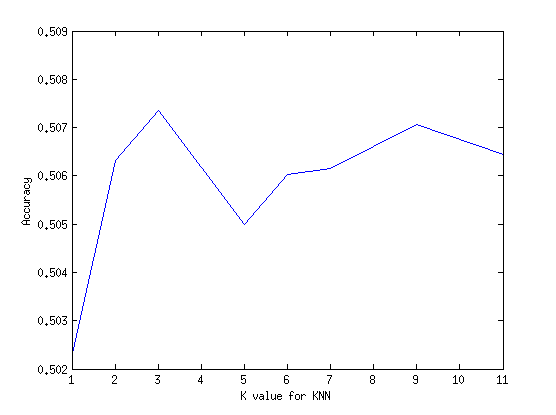
\includegraphics[width = \textwidth]{./img/kforest}
		\parbox{0.95\textwidth}{\caption{Accuracy versus $k_{forest}$ obtained from leave-one-out cross validation. $k_{forest} = 9$ was chosen. \label{fig:Kforest}}}
	\end{subfigure}
	\begin{subfigure}[t]{0.33\textwidth}
		\centering
		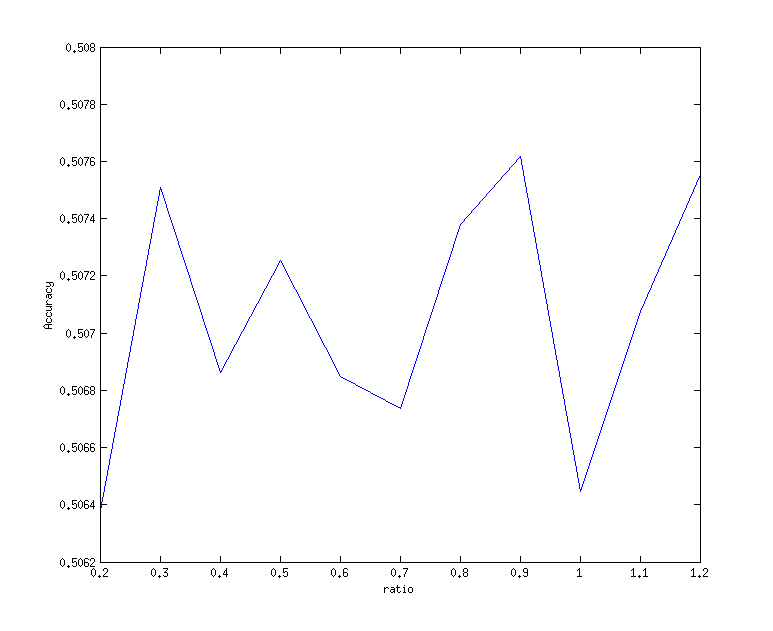
\includegraphics[width = \textwidth]{./img/ratio}
		\parbox{0.95\textwidth}{\caption{Accuracy versus true/false points ratio obtained from leave-one-out cross validation. A ratio  of 0.5 was chosen. \label{fig:ratio}}}
	\end{subfigure}
	\caption{}
\end{figure}

Figure \ref{fig:Kbag} shows the accuracy of the final segmentations of the validation images with respect to the bag of words model parameters. 
For this test, the parameters for the random forest, $k_{forest}$ and ratio, were set to 7 and 0.7 respectively. 
We chose a set of parameters that produced a high accuracy result and did not have a sharpe drop in accuracy for neighboring parameter values. We considered this as an indicator of stability in that it will generalize well to test data.
Consequently, we chose $k_{bag} = 15$, and $k_{hist} = 7$ as these parameters satisfy these properties.

The next parameter we validated was the number of nearest neighbor images on which to train the random forest, $k_{forest}$. 
Figure \ref{fig:Kforest} shows the result of the leave-one-out cross validation on this parameter. The relative magnitude of values in the plot show that accuracy is roughly constant for all $k_{forest}$ except for value 1, for which it is markedly decreased. 
While this plot shows no conclusive reason to choose one $k$ value over another, high $k$ values result in more data points and thus should decrease the variability of the results. 
However, larger values of $k_{forest}$ such as 11 or 13, resulted in unacceptably slow training times. 
Therefore, we chose $k_{forest} = 9$ as it represented an acceptable compromise between these features.

The last varied parameter was the ratio of sampled true points to false points used in the training data for the random forest.
The ratio parameter is of vital importance, as the graph structure proposed in section \ref{sec:labprop} results in a far greater number of same-labeled superpixel pairs than differently-labeled superpixel pairs.
Without this parameter, all tested classifiers tended to fit to the positive labeled points almost exclusively, resulting in high precision and recall but very low specificity. 
However, for our application low specificity is extremely undesirable, as a false-positive, resulting in the classifier propagating a label when it should not , can only degrade the segmentation. By randomly sampling the true points in order to balance the number of trues and falses, all the classifiers we tested, were able to more easily find a decision boundary with high that did not compromise recall too much.  
From the result of cross-validation on this parameter, shown in figure \ref{fig:ratio}, we conclude that a ratio of 0.8 is ideal.


\subsection{Experimental Setup}

Once we obtained the optimal parameters via the procedure described above, we proceeded to test the segmentation algorithm on the 120 images in the test set. We also compare the performance of this approach when training the random forest and bag of words model on the $k-$most similar training images (based on GIST feature representation) versus training on all of them.

Our testbed process iterated through all images in the test set, obtained their prior, and final, post-propagation, segmentations. Then, the process calculated accuracy scores and confusion matrices, across all images, for the prior and the final segmentations and a confusion matrix for the changed superpixels across all images. 

\subsection{Observations}
\label{sec:Observations}

\begin{figure}[htb]
\centering
	\begin{subfigure}[t]{0.19\textwidth}
		\centering
		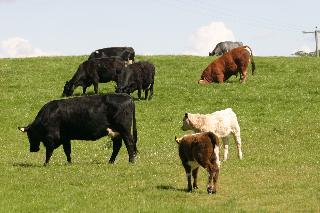
\includegraphics[width = \textwidth]{./img/1_11_s.png}
		\parbox{.95\textwidth}{\caption{Original Image \label{fig:orig_good}}}
			\end{subfigure}
	\begin{subfigure}[t]{0.19\textwidth}
		\centering
		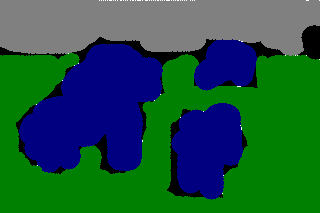
\includegraphics[width = \textwidth]{./img/1_11_s_GT.png}
		\parbox{0.95\textwidth}{\caption{Ground Truth \label{fig:GT_good}}}
	\end{subfigure}
	\begin{subfigure}[t]{0.19\textwidth}
		\centering
		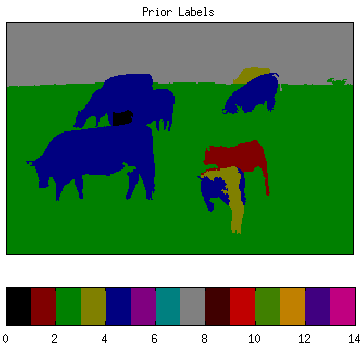
\includegraphics[width = \textwidth]{./img/1_11_s_prior.png}
		\parbox{0.95\textwidth}{\caption{Prior Segmentation \label{fig:prior_good}}}
	\end{subfigure}
	\begin{subfigure}[t]{0.19\textwidth}
		\centering
		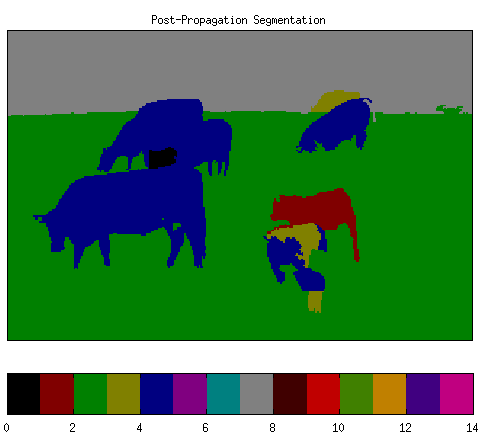
\includegraphics[width = \textwidth]{./img/1_11_s_final.png}
		\parbox{0.95\textwidth}{\caption{Final Segmentation \label{fig:final_good}}}
	\end{subfigure}
	\begin{subfigure}[t]{0.19\textwidth}
		\centering
		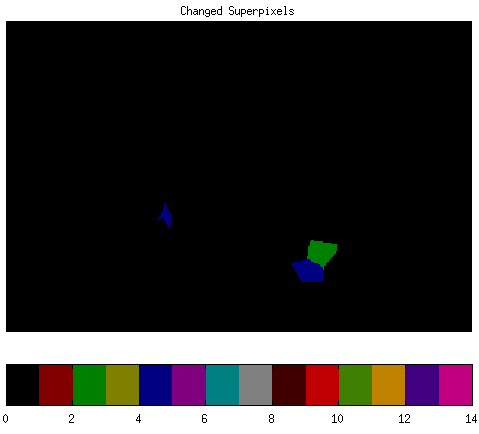
\includegraphics[width = \textwidth]{./img/1_11_s_changed.png}
		\parbox{0.95\textwidth}{\caption{Changed Superpixels \label{fig:changed_good}}}
	\end{subfigure}

	\begin{subfigure}[t]{\textwidth}
		\centering
		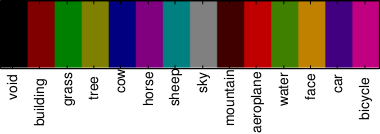
\includegraphics[width = 0.4\textwidth]{./img/legend-rot.png}
	\end{subfigure}
	\caption{Typical result from segmentation algorithm.}
	\label{fig:result_good}
\end{figure}

Figure \ref{fig:result_good} shows a typical result from the segmentation algorithm. In this result, one can see that the error near the hind-legs of the cow on the left, in which a portion of the cow was labeled grass, was successfully fixed using our algorithm. Additionally, the erroneous tree label that appears on the right side of the image is partially replaced by cow and tree labels. However, in this example there is an entire cow mislabeled as a building (in red). Our algorithm is not able to correct a mistake such as this, because it can only propagate existing labels and cannot assign labels by inferring which label would be most probable given the label of the lower entropy superpixel. Our attempted Markov logic network approach should have been able to perform this task, but as mentioned earlier, this approach was infeasible due to memory constraints.

\begin{figure}[htb]
\centering
	\begin{subfigure}[t]{0.33\textwidth}
		\centering
		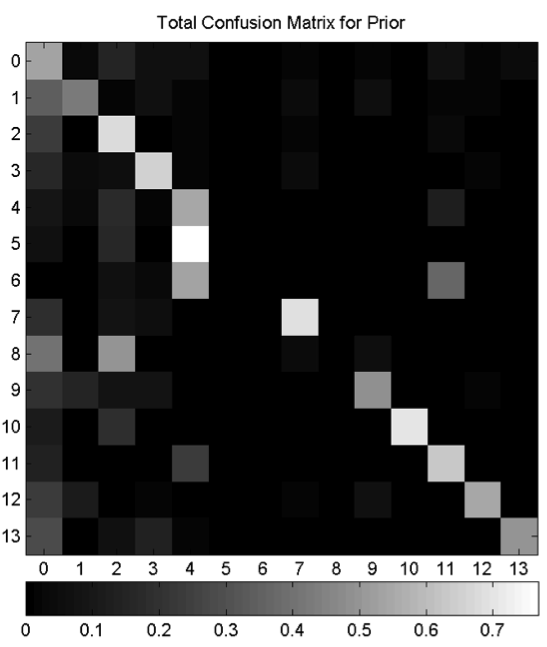
\includegraphics[width = \textwidth]{./img/priorconfuse.png}
		\parbox{.95\textwidth}{\caption{Prior Segmentation. \label{fig:confuse_prior}}}
			\end{subfigure}
	\begin{subfigure}[t]{0.33\textwidth}
		\centering
		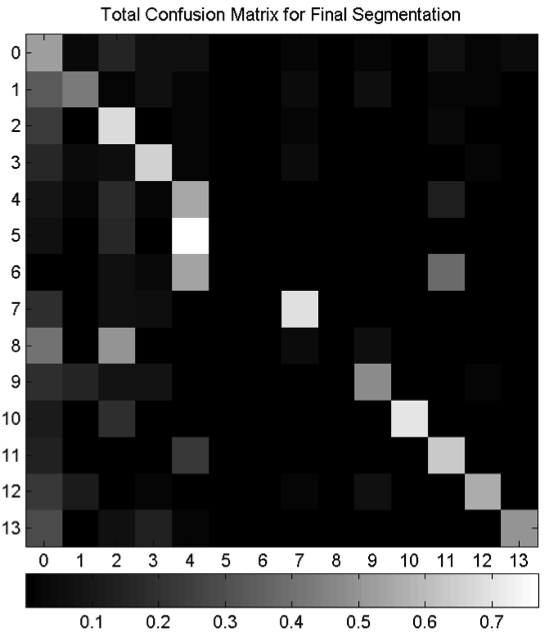
\includegraphics[width = \textwidth]{./img/finalconfuse.png}
		\parbox{0.95\textwidth}{\caption{Final Segmentation \label{fig:confuse_final}}}
	\end{subfigure}
	\begin{subfigure}[t]{0.33\textwidth}
		\centering
		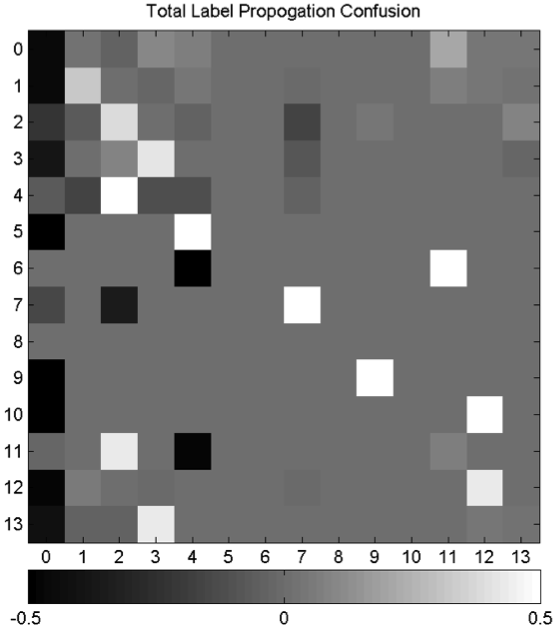
\includegraphics[width = \textwidth]{./img/changeconfuse}
		\parbox{0.95\textwidth}{\caption{Changed Labels \label{fig:confuse_change}}}
	\end{subfigure}
	\caption{Confusion Matrices}
	\label{fig:confuse}
\end{figure}

The overall effect of our label propagation method can be seen in figure \ref{fig:confuse}. This figure shows the confusion matrices for the final segmentation (\ref{fig:confuse_final}), the prior segmentation (\ref{fig:confuse_prior}), and the changed superpixels (\ref{fig:confuse_change}). The confusion matrices for the final and prior segmentations show how, across all test images, our algorithm classified pixels, versus how they are classified in the ground truth images. Specifically, the value  of the $i,j^\textrm{th}$ element in the matrix corresponds to the ratio of instances where our classifier labeled pixels as $j$, when they are labeled $i$ in the ground truth image over the total number of appearances of the $i^\textrm{th}$ label in the dataset. Ideally, this matrix should be diagonal, as this would correspond to perfect agreement between the produced semantic segmentations and the ground truth images. As one can see in the figure the confusion matrices calculated from the result of our test are, for the most part diagonal. 

We can then subtract these confusion matrices to arrive at the confusion matrix for the changed labels. The light elements in this confusion matrix correspond to label co-occurrences of ground truth and final labelings that have increased, while the black regions denote co-occurrences that have decreased. This confusion matrix shows the increases in correctly labeled classes as white elements along its diagonal. It is important to note the many negative elements in the first column of the matrix. These correspond to decreases in the number of labels classified as void in the final segmentations versus the prior segmentations.

From these confusion matrices we can calculate the accuracy of the prior segmentation, the final segmentation, and the accuracy of the changed superpixels. This metric is computed via the following formula:

\begin{equation}
	accuracy = \frac{\mathrm{trace}(A)}{n}
\end{equation}

Where $A$ is a confusion matrix and $n$ is the total number of pixels across all images. We found that the accuracy of our prior segmentations, across all images, was $56.78\%$ while the accuracy of our final segmentations was $56.88\%$. Therefore the improvement in our accuracy was $0.17\%$. This corresponds to a net of roughly 60 superpixels changed correctly across all the test images, a reasonable number considering that some of the prior segmentations do not need improvements.

Another experiment we conducted compared the performance of a segmentation derived from a prior trained on all the images in the training set to a segmentation derived from a prior trained on the $k$-NN images (in terms of distance in GIST feature space) in the training set. The accuracy of the segmentation when using all images for training was $48\%$, a decrease of $13\%$ compared to accuracy obtained by training the prior on the $k$-NN images $(56.88\%)$. The decrease in segmentation accuracy that results from training on all the images stems from the inseparability of all the classes in the feature space. However, when just the $k$-NN are considered, the number of classes that must be separated drops significantly, from 14 to often just 2 or 3, because the $k$-NN images are mostly comprised of the same few labels as the test image. However, one potential downside of this approach is that if a label contained in the test image does not appear in the $k$-NN images, the produced semantic segmentation can never contain this label. In practice, this does not appear to be a problem, as evidenced by the large improvement in accuracy obtained by training on the $k$-NN.
%------------------------------------------------------------------------------------------

\section{Conclusion}
\label{sec:Conclusion}
We have experimented with a label propagation method for semantic segmentation and presented a very simple segmentation algorithm for obtaining a prior. The results, however, show that our approach cannot fix major errors in the prior. A better prior may certainly give much better results. State of art methods (eg. \cite{urtasun}) in this field out perform the results that we have presented. One reason for the bad results could be

Random forests and the baseline use aggregates of local statistics for predicting semantics or relative semantics between image patches. There is a chance that both approaches are right at the same places and wrong at the same places too and in these cases label propagation will not help. Therefore, even though our random forest achieves precision, recall and specificity values $\ge 80\%$, we do not make much progress in terms of improving the baseline.

\bibliographystyle{plain}
\bibliography{final_report}

\end{document}
